% F035 指数幂的运算法则｜06 快记 + 快用
\clearpage
\begin{summarybox}
    \textbf{\textcolor{CSummary}{一分钟记住：先看长什么样，再决定怎么运算}}\par
    \begin{description}[style=nextline,leftmargin=2.3em,itemsep=0.35em]
        \item[\textbf{同底相乘，指数加：}]
        \[a^ma^n=a^{m+n}\quad(\text{两串接一起}).\]
        \item[\textbf{幂的乘方，指数乘：}]
        \[(a^m)^n=a^{mn}\quad(\text{每组 $m$ 个，有 $n$ 组}).\]
        \item[\textbf{积的乘方，分别乘：}]
        \[(ab)^m=a^mb^m\quad(\text{每个因子都不能漏}).\]
    \end{description}
    \begin{center}
    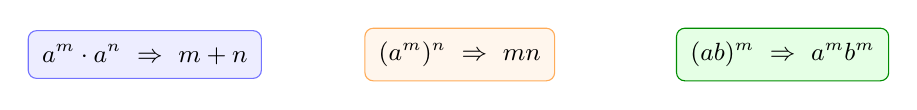
\begin{tikzpicture}[font=\small]
        \node[draw=blue!55,fill=blue!7,rounded corners=3pt,inner sep=5pt] at (0,0) {$a^m\cdot a^n\ \Rightarrow\ m+n$};
        \node[draw=orange!65,fill=orange!7,rounded corners=3pt,inner sep=5pt] at (4.0,0) {$(a^m)^n\ \Rightarrow\ mn$};
        \node[draw=green!55!black,fill=green!10,rounded corners=3pt,inner sep=5pt] at (8.1,0) {$(ab)^m\ \Rightarrow\ a^mb^m$};
    \end{tikzpicture}

    \end{center}

    \textbf{\textcolor{CSummary}{做题最快三步}}\par
    \begin{enumerate}[leftmargin=*,itemsep=0.25em,topsep=0.3em]
        \item \textbf{认结构：} 并排相乘？括号外乘方？还是积的乘方？
        \item \textbf{查条件：} 实数指数优先确保底数为正；出现 $0$ 或负底数要特别检查。
        \item \textbf{选路径：} 能化同底就化同底，能按同指数合并底数也可以，最后再计算。
    \end{enumerate}

    \textbf{\textcolor{CSummary}{最容易丢分的两件事}}\par
    $a^m+a^n$ \textbf{不能}直接把指数相加；$(a+b)^m$ \textbf{不能}照搬积的乘方。

    \textbf{\textcolor{CSummary}{一句话回扣：}}\textbf{连在一起数相加，分成几组数相乘，括号是乘积就分别乘方。}
\end{summarybox}
